\section{Forward vs. Backward}

\paragraph{Problem}
Implement and compare Repeated Forward A* and Repeated Backward A* with respect
to their runtime or, equivalently, number of expanded cells. Explain your
observations in detail, that is, explain what you observed and give a reason
for the observation. Both versions of Repeated A* should break ties among cells
with the same f-value in favor of cells with larger g-values and remaining ties
in an identical way, for example randomly.

\paragraph{Solution}

As the Table \ref{tbl:rfa-rba} shows,the repeat backward a* search expands
more notes extremely. In average, each map, RBA* take more than 15 times time,
namely the expanded notes, than RFA*. In addition, in each procedure of compute
the path, RBA* also expands notes more than 10 times than RFA*. So, The
efficiency of RBA* is much worse than that of RFA*.

\begin{table}[h!]
\centering
\caption{Result of Repeated Forward A* and Repeated Backward A*}
\begin{tabular}{|l|l|l|l|l|}
\hline
Algorithm & Aver. Expa/M & aver. Expa/P & Aver. Expl/M & Aver. Expl/P \\
\hline
RFA* & 8847.88 & 92.44 & 25461.42 & 267.68 \\
\hline
RBA* & 133043 & 1272.54 & 266050.76 & 2551.44 \\
\hhline{|=|=|=|=|=|}
Algorithm & Aver. Moves & Aver. Count & Aver. Optimal & Aver. Ratio \\
\hline
RFA* & 335.72 & 88.2 & 198.6 & 1.6852 \\
\hline
RBA* & 390.88 & 103.4 & 198.6 & 1.9626 \\
\hline
\end{tabular}
\label{tbl:rfa-rba}
\end{table}

The reason of this is that, When computing the path, RFA* always can know which
cells is blocked, thus it can avoid the cells blocked immediately. In contrast,
RBA* is search from the goal, and the most cells near goal is unknown. So RBA*
will find unblocked cells very late, which may result in that RBA* has to
compute another path in a early note it expanded. So RBA* will cost more time,
or expands more cells to find the shortest path.

\begin{figure}
  \centering
  \begin{subfigure}[b]{0.45\textwidth}
    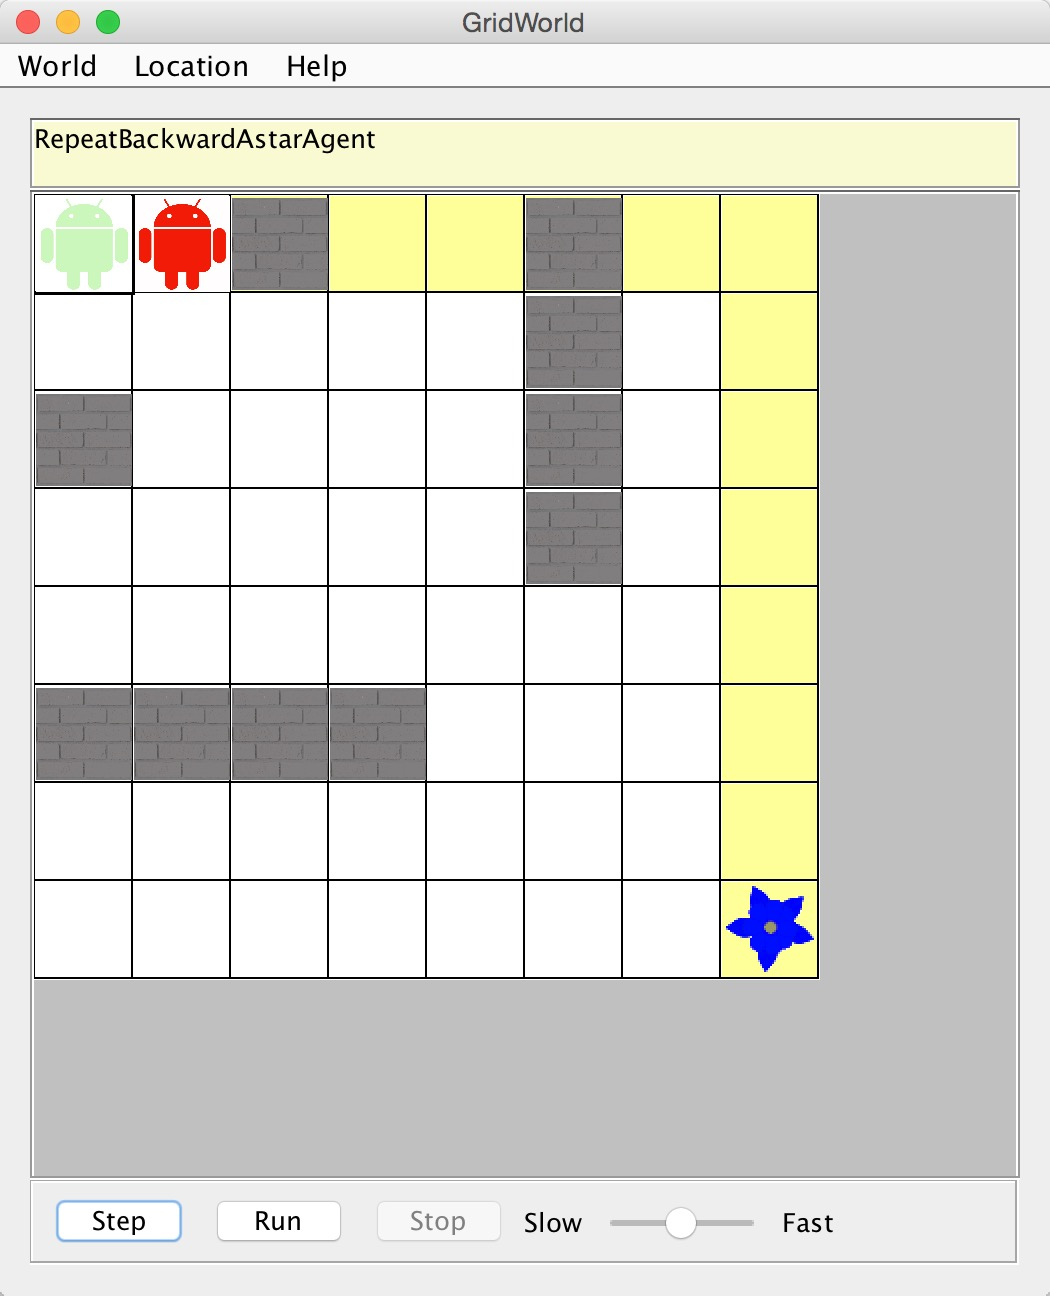
\includegraphics[width=\textwidth]{RBA-1.png}
    \caption{RBA* before computing}
    \label{fig:p3-rba-1}
  \end{subfigure}
  \begin{subfigure}[b]{0.45\textwidth}
    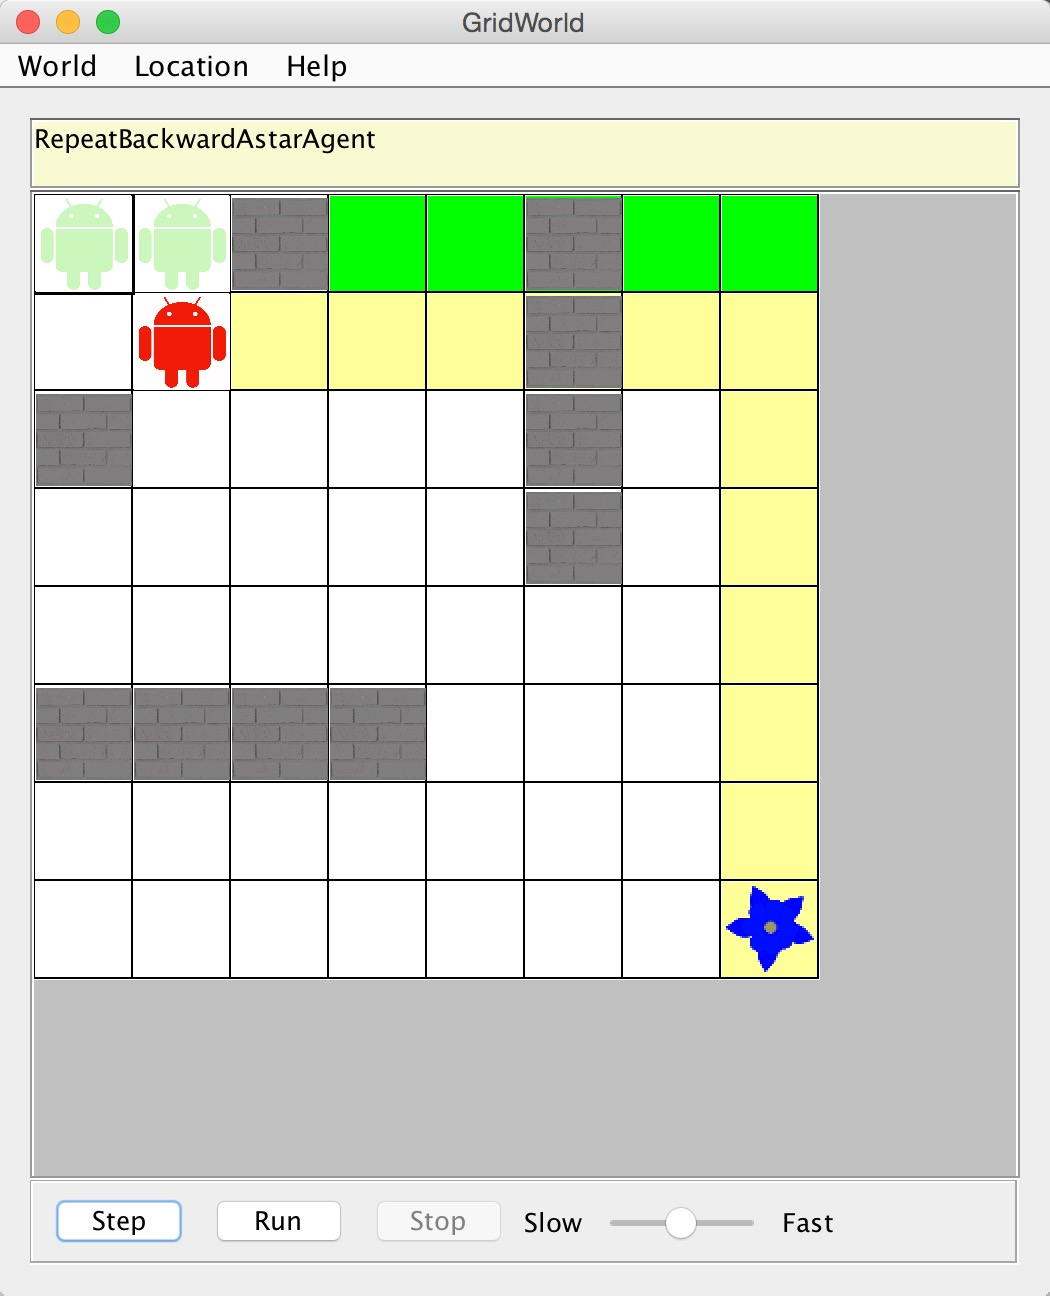
\includegraphics[width=\textwidth]{RBA-2.png}
    \caption{RBA*  after computing}
    \label{fig:p3-rba-2}
  \end{subfigure}
  \caption{Example of RBA* procedure for computing path}
  \label{fig:p3-rba}
\end{figure}

For example, in the Figure \ref{fig:p3-rba}, denote each cell as c(i,j), i,j
is the row number and column number from 1 to 8. In the figure (a), the agent
encounter a blocked cell c(1,3), then it has to compute the path again. Using
RBA* search, it will compute the path from goal. When the compute procedure
reach c(1,4) along the yellow path,  near the agent, it will find its adjacent
c(1,3) is blocked. Then it has to turn down to c(2,4). However, when the cell
c(2,8) expanded, its left cell c(2,7) is added to open-list. And f(c(2,7)) =
h(c(2,7)) + g(c(2,7)) = 7 + 7 = 14. While f(c(2,4)) = h(c(2,4)) = 4 + 12 =16.
So, the procedure will chose c(2,7) to expand. Thus there will be a new path in
this procedure of compute path, like the Figure \ref{fig:p3-rba}.

\begin{figure}
  \centering
  \begin{subfigure}[b]{0.45\textwidth}
    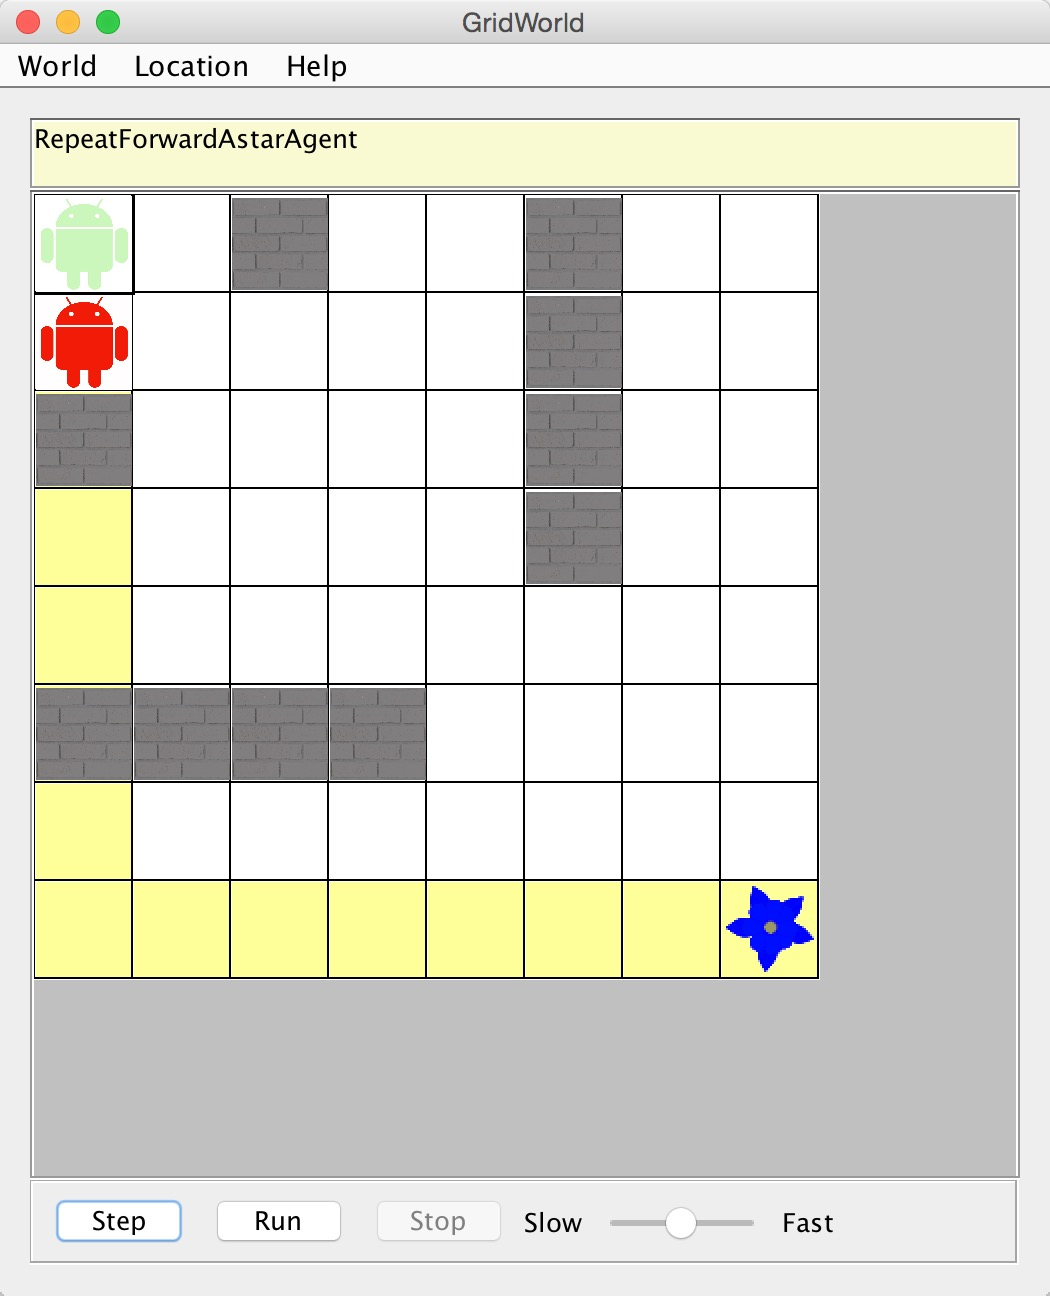
\includegraphics[width=\textwidth]{RFA-1.png}
    \caption{RFA* before computing}
    \label{fig:p3-rfa-1}
  \end{subfigure}
  \begin{subfigure}[b]{0.45\textwidth}
    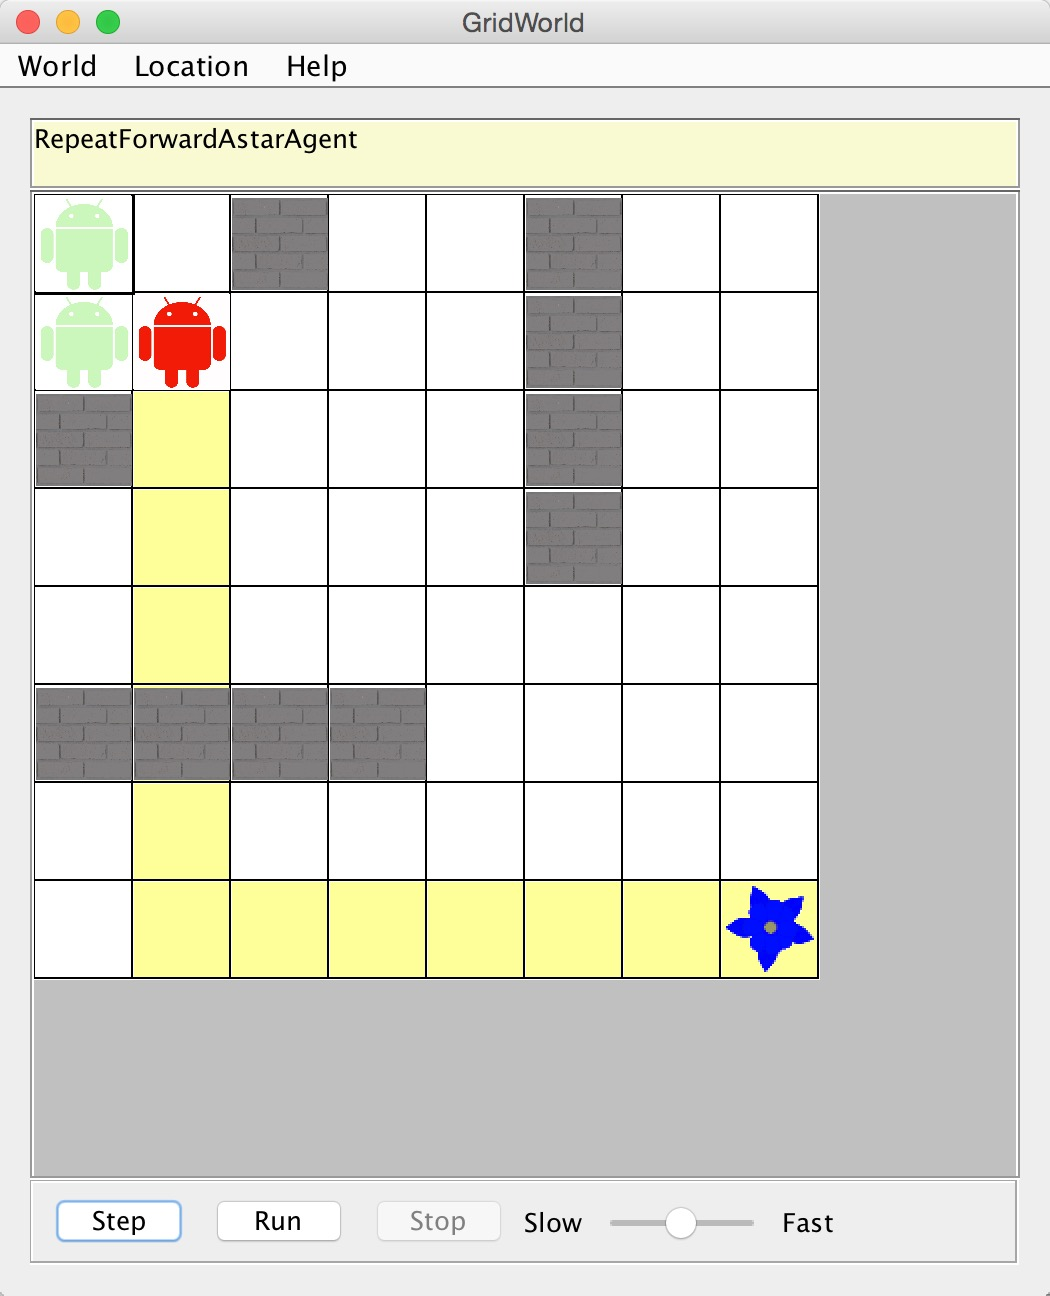
\includegraphics[width=\textwidth]{RFA-2.png}
    \caption{RFA* after computing}
    \label{fig:p3-rfa-2}
  \end{subfigure}
  \caption{Example of RFA* procedure of computing path}
  \label{fig:p3-rfa}
\end{figure}

In contrast, such as Figure \ref{fig:p3-rfa} shows, when RFA* computes the path,
it will find c(3,1) is blocked immediately, thus it will avoid to add it to the
shortest path at once.Then it will not expand extra cells.

